\chapter{Common Linux Types and Locks}

With 25 millions LOC you can be sure that there are many areas of the kernel that implement structures, locks and so on in very similar ways. To avoid this duplication, there are several types and structures provided by the kernel that kernel developers can use. As you browse the kernel code you'll see lots of references to linked lists, containers and so on XXX

This section describes the most common types and gives examples of how they're used.

% https://medium.com/@414apache/kernel-data-structures-linkedlist-b13e4f8de4bf - covers most of them

%-------------------------------------------------------------------------------------------------------------------------------------------------------------------------

\section{Lists}

xxx

\begin{lstlisting}
struct list_head {
    struct list_head *next, *prev;
};
\end{lstlisting}

\noindent
xxxx

\begin{lstlisting}
#define [*\bfseries list\_for\_each*](pos, head) \ 
    for (pos = (head)->next; pos != (head); pos = pos->next)
\end{lstlisting}

\noindent
xxxx


%---------------------------------------------------------------------------------------------------------------------------------------------------------------------------

\subsection{An Unusual List Example}

In some structures, the list element is not at the start of the structure which can make it a challenge to debug. Take the \cf{mount} structure as an example. The list of mounted filesystems is referenced by the global variable \cf{super\_blocks}. This is a list HEAD (?) structure which points to the front element of the list and the last. Each element is of type \cf{struct super\_block}. Inside this structure we have:

\begin{lstlisting}
struct list_head    s_mounts;   /* list of mounts; 
                                 _not_ for fs use */
\end{lstlisting}

\noindent
In \cf{gdb} you can use a Linux helper function to display the mounted filesystem list. For each, it displays the \cf{super\_block} structure as well as one of the \cf{mount} structures. Section XXX will explain the "one vs many" issue. For now, let's look at one entry:

\begin{lstlisting}
(gdb) [*\bfseries lx-mounts*]
mount            super_block      devname    path fstype options
...
0xf...812f3ea500 0xf...8127b7c800 /dev/loop8 /mnt spfs   rw,r...
\end{lstlisting}

\noindent
Taking the address of the \cf{super\_block} structure, we can display the \cf{s\_mounts} field as follows:

\begin{lstlisting}
(gdb) [*\bfseries set \$sb = (struct super\_block *)0xffff888127b7c800*]
(gdb) [*\bfseries p \$sb->s\_mounts*]
$3 = {
  next = 0xffff88812f3ea578,
  prev = 0xffff888101952cf8
}
\end{lstlisting}

\noindent
Ignoring the \cf{prev} element for now, the \cf{next} field points to a \cf{mount} structure but look at the address versus the address displayed by \cf{lx-mounts}:

\begin{lstlisting}
0xffff88812f3ea5[*\bfseries 00*]   # displayed by lx-mounts
0xffff88812f3ea5[*\bfseries 78*]   # what's in s_mounts
\end{lstlisting}

\noindent
There is a difference of \cf{0x78} between both addresses. This is because the linked list is actually \textbf{through?} the \cf{mnt\_instance} field:

\begin{lstlisting}
struct list_head  mnt_instance;  
\end{lstlisting}

\noindent
which is at an offset of 0x78 bytes:

\begin{lstlisting}
(gdb) [*\bfseries p \&\$mount->mnt\_instance*]
$39 = (struct list_head *) 0xffff88812f3ea578
\end{lstlisting}

\noindent
If you search for \cf{mnt\_instance} in the kernel \cf{fs} directory you will find code that walks this list:

\begin{lstlisting}
[*\bfseries list\_for\_each\_entry*](mnt, &sb->s_mounts, mnt_instance) {
    /* process each structure */
}
\end{lstlisting}

\noindent
Internally, a call will be made to \cf{container\_of} which will be described in the next section \textbf{(or earlier/??????)}

%%%%%%%%%%%%%%%%%%%%%%%%%%%%%%%%%%%%%%%%%%%%%%%%%%%%%%%%%%%%%%%

\section{Locks}

xxx

%%%%%%%%%%%%%%%%%%%%%%%%%%%%%%%%%%%%%%%%%%%%%%%%%%%%%%%%%%%%%%%

\section{The \cf{xarray} Structure}

XXX - i\_pages from the address\_space structure points is of type "struct xarray". it's a list of all cached pages.

See https://docs.kernel.org/core-api/xarray.html for information

and https://lwn.net/Articles/745073/

to see actual contents, will need to call kmap() -  https://stackoverflow.com/questions/31966298/can-we-access-memory-through-a-struct-page-structure. Also kmap\_atomic()

\textbf{need to come back here once I understand it ... there is a "virtual" field but it's configurable. So how does the page get mapped in?}

%%%%%%%%%%%%%%%%%%%%%%%%%%%%%%%%%%%%%%%%%%%%%%%%%%%%%%%%%%%%%%%

\subsection{The Big Kernel Lock (BKL}

As Linux transitioned to SMP (Symmetric Multi-Processing) architectures, a temporary solution was needed until more kernel components could be changed to support fine-grain locking. This \textit{solution} was called the Big Kernel Lock (BKL) which was a global spin-lock 

\begin{lstlisting}
lock_kernel();

/*
 * Critical section, synchronized against all other BKL users...
 * Note, you can safely sleep here and the lock will be transparently
 * released. When you reschedule, the lock will be transparently
 * reacquired. This implies you will not deadlock, but you still do
 * not want to sleep if you need the lock to protect data here!
 */

unlock_kernel();
\end{lstlisting}

\noindent
xxx

At the kernel there were three functions that could be called:

\begin{itemize}
	\item \cf{lock\_kernel()} -- acquire the BKL
	\item \cf{unlock\_kernel()} -- release the BKL
	\item \cf{kernel\_locked()} -- returns non-zero if the BKL is held and zero otherwise
\end{itemize}

\noindent
The BKL was finally removed it in 2011 in kernel version 2.6.39. 

%%%%%%%%%%%%%%%%%%%%%%%%%%%%%%%%%%%%%%%%%%%%%%%%%%%%%%%%%%%%%%%

\subsection{Local Locks}

xxx

\subsection{Semaphores}

xxx

\subsection{Mutexes}

xxx

%-------------------------------------------------------------------------------------------------------------------------------------------------------------------------

\section{Black-Red Trees}

Black-red trees, often abbreviated to \textit{rbtrees}, are a type of self-balancing binary search tree and are used for storing sortable key/value data pairs.

\begin{table}[h]
\begin{tabular}{ll}
\parbox[l]{0.6in}{
\includegraphics[scale=0.8]{figures/src-xref.pdf}} & \parbox[l]{4in}{\small{You can find the Linux rbtree implementation in \cf{lib/rbtree.c}}}
\end{tabular}
\end{table}

\noindent
Linux has \textit{augmented rbtrees}

An \textit{nterval tree} is an example of augmented rbtree

From lwn:

\begin{quote}
There are a number of red-black trees in use in the kernel. The anticipatory, deadline, and CFQ I/O schedulers all employ rbtrees to track requests; the packet CD/DVD driver does the same. The high-resolution timer code uses an rbtree to organize outstanding timer requests. The ext3 filesystem tracks directory entries in a red-black tree. Virtual memory areas (VMAs) are tracked with red-black trees, as are epoll file descriptors, cryptographic keys, and network packets in the "hierarchical token bucket" scheduler.
\end{quote}

%-------------------------------------------------------------------------------------------------------------------------------------------------------------------------

\section{Wrapping Structures With \cf{container\_of}}\label{container-of}

% https://stackoverflow.com/questions/15832301/understanding-container-of-macro-in-the-linux-kernel
%
% the above has great explanations but is it worth it? Just expand the part about pointer arithmetic.

There are many structures in the kernel that embed other structures, particularly those that are linked together in a linked list. This is where the \cf{container\_of()} macro comes in useful. The basic idea is that we have one structure embedded (or contained within) another structure. The embedded structure is often one member of a linked list or tree structure. In this example, we have a linked list of VFS inodes and each is embedded in a structure used by the filesystem that allows it to get to filesystem-specific information about this file.

\begin{figure}
	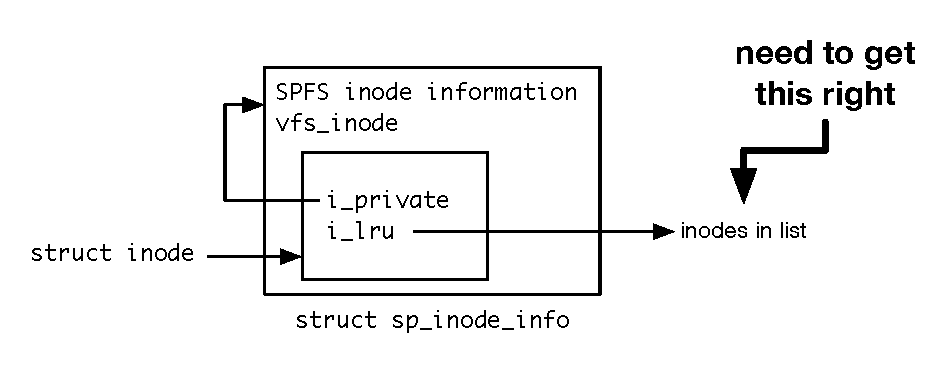
\includegraphics[scale=0.6]{figures/containerof.pdf}
	\centering
	\caption{Using \cf{container\_of()} to get to the "\textit{containing}" structure}
	\label{fig:containerof}
\end{figure}

\noindent
Let's take a look at this confusing looking macro:

\begin{lstlisting}
/**
 * container_of - cast a member of a structure out to the 
 * containing structure
 * @ptr:    the pointer to the member.
 * @type:   type of the container struct this is embedded in.
 * @member: the name of the member within the struct.
 *
 */
#define [*\bfseries container\_of*](ptr, type, member) ({                    \
    void *__mptr = (void *)(ptr);                             \
    static_assert(__same_type(*(ptr), ((type *)0)->member) || \
              __same_type(*(ptr), void),                      \
              "pointer type mismatch in container_of()");     \
    ((type *)(__mptr - offsetof(type, member))); })
\end{lstlisting}

\noindent
It really does look like something you'd see during an interview when they get into that annoying programming phase! But the idea is actually very simple and the function is basic pointer arithmetic. Let's take inodes as an example. Inodes, as seen in section \ref{inodes}, are structures representing files both in-core and on disk, thus an incore inode and a disk inode. When a file is opened, the disk inode will be brought into memory and the filesystem will likely cache all or part of it. The Linux inode is used by the VFS layer and will be passed to the filesystem through many of the different VFS to filesystem functions. Often, the first thing the filesystem will do is get hold of its disk inode from the incore inode.

The Linux inode also have a field called \cf{i\_private} which has traditionally been used to reference filesystem-specific information. In this case, when the inode is being initialized, the filesystem would allocate its own inode structure (or equiavelent) and set \cf{i\_private} to point to this structure. For example:

\begin{lstlisting}
struct sp_inode_info      *spi;
...
inode->i_private = spi;
\end{lstlisting}

\noindent
and then reference it using a macro such as:

\begin{lstlisting}
#define ITOSPI(inode)   (struct sp_inode_info *)&inode->i_private
\end{lstlisting}

\noindent
Take the following BFS filesystem code fragment as an example: \textbf{XXX---replace with SPFS code after starting to use container\_of}

\begin{lstlisting}
static void bfs_evict_inode(struct inode *inode)
{
    ...
    struct bfs_inode_info *bi = BFS_I(inode);
    ...
\end{lstlisting}

\noindent
The \cf{BFS\_I} function takes the incore inode as an argument and returns a pointer to BFS specific inode information for this file:

\begin{lstlisting}
static inline struct bfs_inode_info *BFS_I(struct inode *inode)
{
    return container_of(inode, struct bfs_inode_info, vfs_inode);
}
\end{lstlisting}

\noindent
Here is the definition of the \cf{bfs\_inode\_info} structure:

\begin{lstlisting}
struct bfs_inode_info {
    unsigned long i_dsk_ino; 
    unsigned long i_sblock;
    unsigned long i_eblock;
    [*\bfseries struct inode vfs\_inode;*]
};
\end{lstlisting}

\noindent
The Linux inode is embedded in this structure which can be described as the \textit{container of} the Linux inode.

This is very commonly used in the Linux kernel. I found over 17,000 references to \cf{container\_of} in C files. 

Section \textbf{kdgb-inodelist} shows how inodes are linked together and associated with a specific \cf{super\_block} structure representing a specific mount point. 

%-------------------------------------------------------------------------------------------------------------------------------------------------------------------------

\section{Semaphores, Mutexes, And Lockless Algorithms}

You will need an lwn.net subscription to be able to read this article.

\begin{table}[h]
\begin{tabular}{lcl}
\parbox[r]{0.5in}{
\includegraphics[scale=0.15]{figures/url.png}} & \parbox[l]{0.55in}{URL \arabic{urls} -- } & \parbox[l]{3in}{\cf{https://tinyurl.com/4y2d3yen}}
\end{tabular}
\end{table}
\stepcounter{urls}
% https://lwn.net/Articles/928026/

some of this list comes from the lwn article so broaden as much as possible

\begin{enumerate}
	\item semaphores vs mutexes history
	\item spinlocks
	\item lockless algorithms
	\item the big lock
	\item early days - nothing but cli() /sti()
	\item SCSI semaphores -> binary semaphores
	\item semaphores on the way out? lwn article
	\item major locks used for FS structures
	\item etc
\end{enumerate}

\noindent 
xxx

%-------------------------------------------------------------------------------------------------------------------------------------------------------------------------

\section{Read-Copy Update (RCU) Synchronization}

RCU (Read-Copy Update) was first implemented RCU in the Sequent DYNIX/ptx operating system and documented in 1998. DYNIX (DYNamic unIX) was a UNIX variant based on 4.2BSD and later System V UNIX designed to run on Intel SMP processors.

The first RCU mechanisms were introduced in Linux back in 2002 as a means to create large-scale scalability improvements by allowing reads to occur concurrently with updates.

The most common use of RCU in the Linux kernel is as an alternative to a read-write locking. Pathname resolution  is one particularly important use case and is described in section \ref{xxx}.

% https://pdos.csail.mit.edu/6.828/2020/readings/rcu-decade-later.pdf - Usenix very detailed

%%%%%%%%%%%%%%%%%%%%%%%%%%%%%%%%%%%%%%%%%%%%%%%%%%%%%%%%%%%%%%%

\section{Conclusion}

There are several different locking primitives over the years and parts of the kernel have been heavily optimized to minimize taking locks unless absolutely necessary to avoid contention on today's multi-processor systems resulting in the loss of performance.

Like most operating systems, Linux took some time to transition from uniprocessor systems (UP) to symmetric multiprocessing (SMP) systems. After starting with the Big Kernel Lock (BKL), the kernel was in time, transitioned to use XXX.

TBD

